\documentclass[Rapport/Playerside/RPI_IF/RPI_IF.tex]{subfiles}
\label{sec:playerside_RPI_IF_design}
\begin{document}
\subsubsection{Design}
I dette afsnit omtalles RPI\_IF boundary klassens design. Klassen er en boundary klasse til RPI(Raspberry Pie) og skal stå for at sende kop status beskeder til RPI'en, når en ændring forekommer. Den skal også stå for at modtage beskeder fra RPI'en, som kan være en farvekode eller en state ændring. I grænsefladeafsnittet i arkitekturen er en mere uddybende beskrivelse af disse beskeder. Protokollen brugt er I2c og til dette formål er en i2c slave komponent brugt i PSoC creators komponent katalog. På figur \ref{fig:I2c_slave} ses denne komponent.
\begin{figure}
    \centering 
    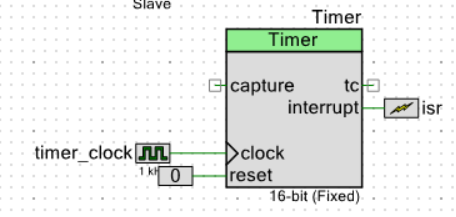
\includegraphics[width=\linewidth]{Softwaredesign/GameController/graphic/gamecontroller_timer.PNG}
    \caption{I2C slave komponent brugt til i2c kommunikationen mellem PSoC playerside og RPI}
    \label{fig:I2c_slave}
\end{figure}
Denne komponent skal initieres, for at se hvordan dette gøres ses RPI\_IF design bilag. I arkitekturen for denne klasse ses, der to funktioner, der er brugt. Det er sendCupStatus og RPI\_IF\_handledata. Her er sendCupStatus den metode, der står for at sende beskeder omkring kop status tilbage til RPI og er brugt af GameController klassen, når den modtager kopstatus ændring fra CupSensor\_IF. For en mere detaljeret beskrivelse ses design bilag for RPI\_IF. Funktionen  RPI\_IF\_handledata står for modtagelsen af state ændringer for playerside samt beskeder omkring ændring af farvekode for begge playersides. I denne metode vil flere metoder fra GameController bruges alt afhængig af, hvilken besked er sendt. For mere information om RPI\_handledata metodens funktion ses RPI\_IF bilag og for mere information om GameController metoderne ses design afsnittet for GameController, samt bilaget dertil.
\end{document}